It is reasonable to consider the ``fragility'' of a birth and death chain through the lens of
recurrence, a mathematical property of Markov chains that categorizes states of a chain based on whether
the chain is expected to return to that state. Further, in the case of chains with infinite states---a
birth and death chain where the states are values of $\N$, for instance---a distinction is drawn between
those states where the expected return time is infinite, and those where the expected return time is
finite.  States are thus called \emph{null-recurrent} or \emph{positive-recurrent}, respectively. In
contrast, a state is called \emph{transient} if the chain cannot be expected to return.

This allows a mathematical characterization of instances in which the chain seems to ``get lost'' from
the origin. For instance, if the origin is classified as a transient state, then a walker starting at
the origin cannot be expected to return to the origin (he may, but not with full probability). In
contrast, if the origin were classified as a recurrent state, then the walker will return with
probability $1$.  Further, if the origin were null-recurrent, the walker may find himself diverging from
the origin for arbitrary periods of time, but will with probability $1$ eventually return. If the origin
were positive-recurrent, then a concrete estimate can be placed on the walker's return time to the
origin.  This is to say that transient states are the ``most lost,'' as there can be no concrete
expectations about a walker's return to such states, nor can concrete estimates be made about how long
returning may take.  Null-recurrent states are still ``somewhat lost,'' though less so than transient
states due to the fact that concrete expectations \emph{can} be made about a walker's return.
Positive-recurrent states are the "least lost'' since a walker can be expected to return within a finite
amount of time.

In order to investigate how recurrence properties impact a chain's ``fragility,'' I first needed to
analyze some specific examples of birth and death chains. In particular, I defined a chain in which the
state-space---the possible positions that the chain can take---is the integers. Then, let
\[
    p(x) = \begin{cases}
        \frac{1}{2+\abs{x}^{-\beta}} & \text{if } x > 0 \\
        1 - \frac{1}{2+\abs{x}^{-\beta}} & \text{if } x < 0 \\
        \frac{1}{2} & \text{if } x = 0
    \end{cases}.
\]
for some $\beta >= 0$, and let $q(x) = 1 - p(x)$. Let $r(x) = 0$. This represents a birth and death
chain that is somewhat biased towards the origin, and in which the limiting probabilities
\[
    \lim_{x \to \infty} p(x) = \lim_{x \to \infty} q(x) = \frac{1}{2}  
\]
and
\[
    \lim_{x \to -\infty} p(x) = \lim_{x \to -\infty} q(x) = \frac{1}{2}.  
\]
Physically, this should represent that a walker at extremely far distances from the origin cannot see
it, and so should step either in the positive direction or in the negative direction with probability
$1/2$. We will refer to this birth and death chain as the \emph{power-distributed birth and death chain}
with parameter $\beta$.

Unfortunately, unlike in the case of stationary Markov chains in which probabilities are independent of
the position---which usually simplifes analysis---the recurrence properties of this birth and death
chain will need to be investigated a different way. I hypothesize, in particular, that if $\beta < 1$,
then the origin in the above chain will be a positive-recurrent state, and that if $\beta > 1$, then the
origin will be a null-recurrent state. In order to develop a stronger intuition about this behavior, I
turned to some numerical simulations in Python, using the NumPy and Matplotlib libraries.

I began by writing a base-class that represents a random walk, from which more specific instances can be
derived. I then developed a birth and death class inherited from the random walk base class. This
implemented the specific probability distribution detailed above. Then, for each $\beta$ in a range of
$\beta$ values---defined by a minimum $\beta$, maximum $\beta$, and $\beta$ step-size---a simulation of
one-million time steps was run, with the origin as the initial position, and the given probability
distributions. Then, using the fact that storage of return times is implemented in the random walk
class, the mean and standard-deviation of the return times was calculated, and plotted using
Matplotlib's \texttt{pyplot} class. In particular, I used the scatter-plot, histogram, and 2-dimensional
histogram functions.

For example, the following plot shows the mean return times of a simulation with $\beta$ values ranging
from $0$ to $3$ with a increments of $0.005$.

\noindent
\begin{figure}[H]
    \begin{center}
        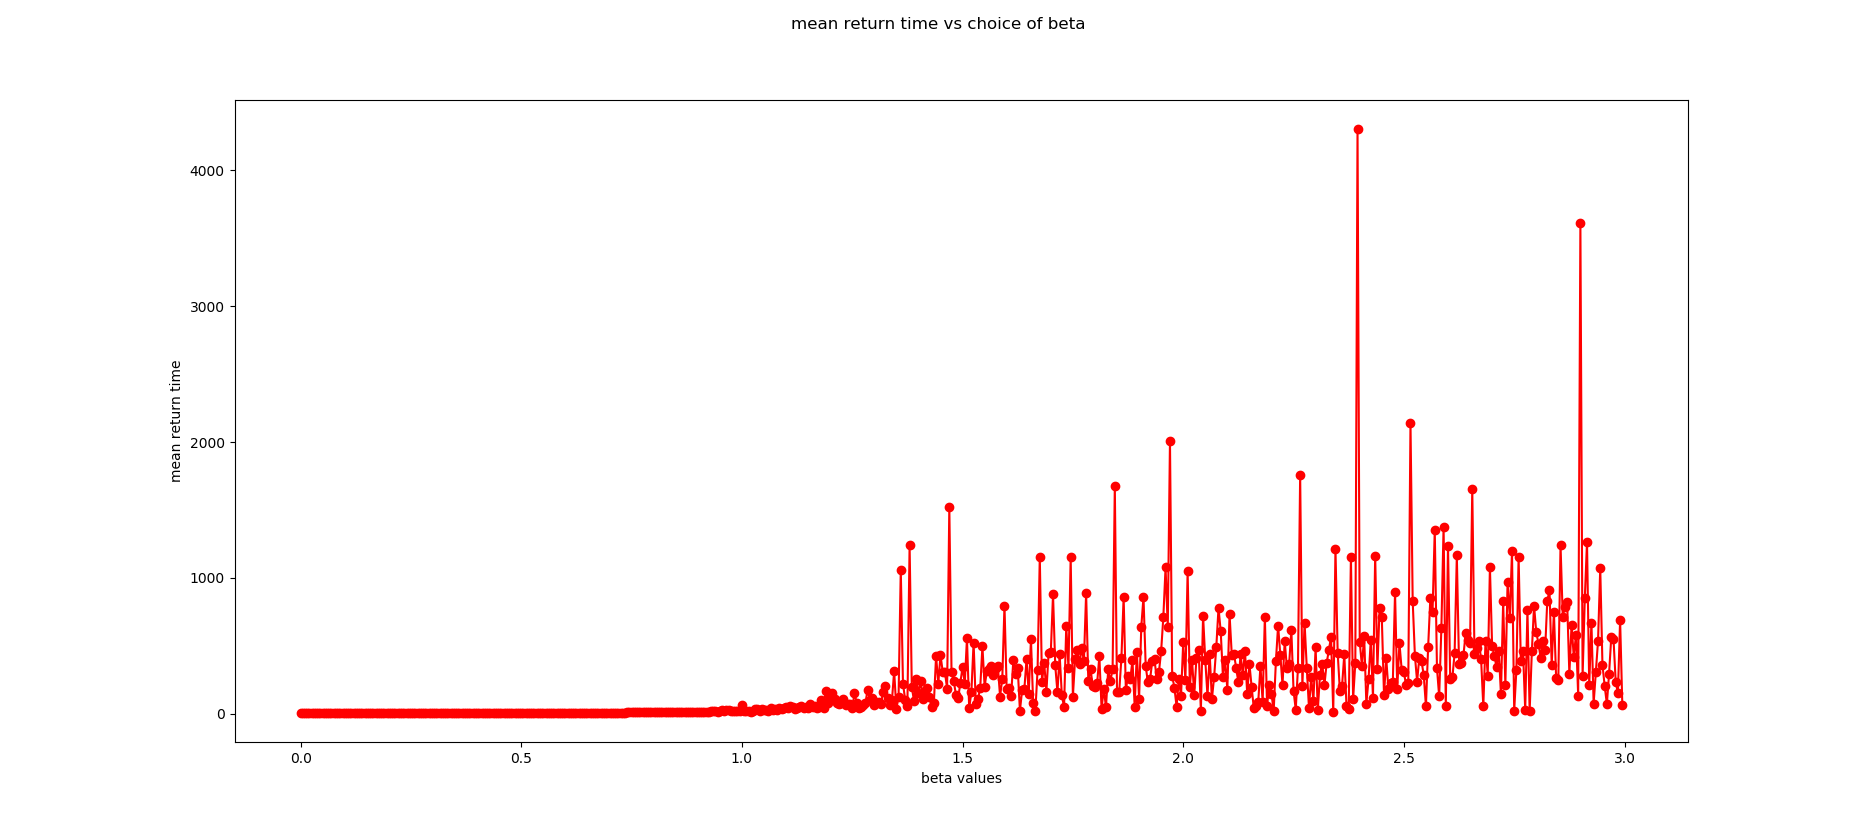
\includegraphics[width=\textwidth]{plots/returntimesplot1.png}
    \end{center}
\end{figure}

Here, it appears as though the mean return times begin to scatter into higher values shortly after
$\beta$ grows beyond $1$, thus supporting that the chains may be getting ``more lost'' more frequently.
This suggests that the origin in the given birth and death chain may be either null-recurrent or
transient when $\beta > 1$ and is, in contrast, positive-recurrent when $\beta < 1$. The corresponding
$2$-dimensional histogram similarly supports this conclusion.

\noindent
\begin{figure}[H]
    \begin{center}
        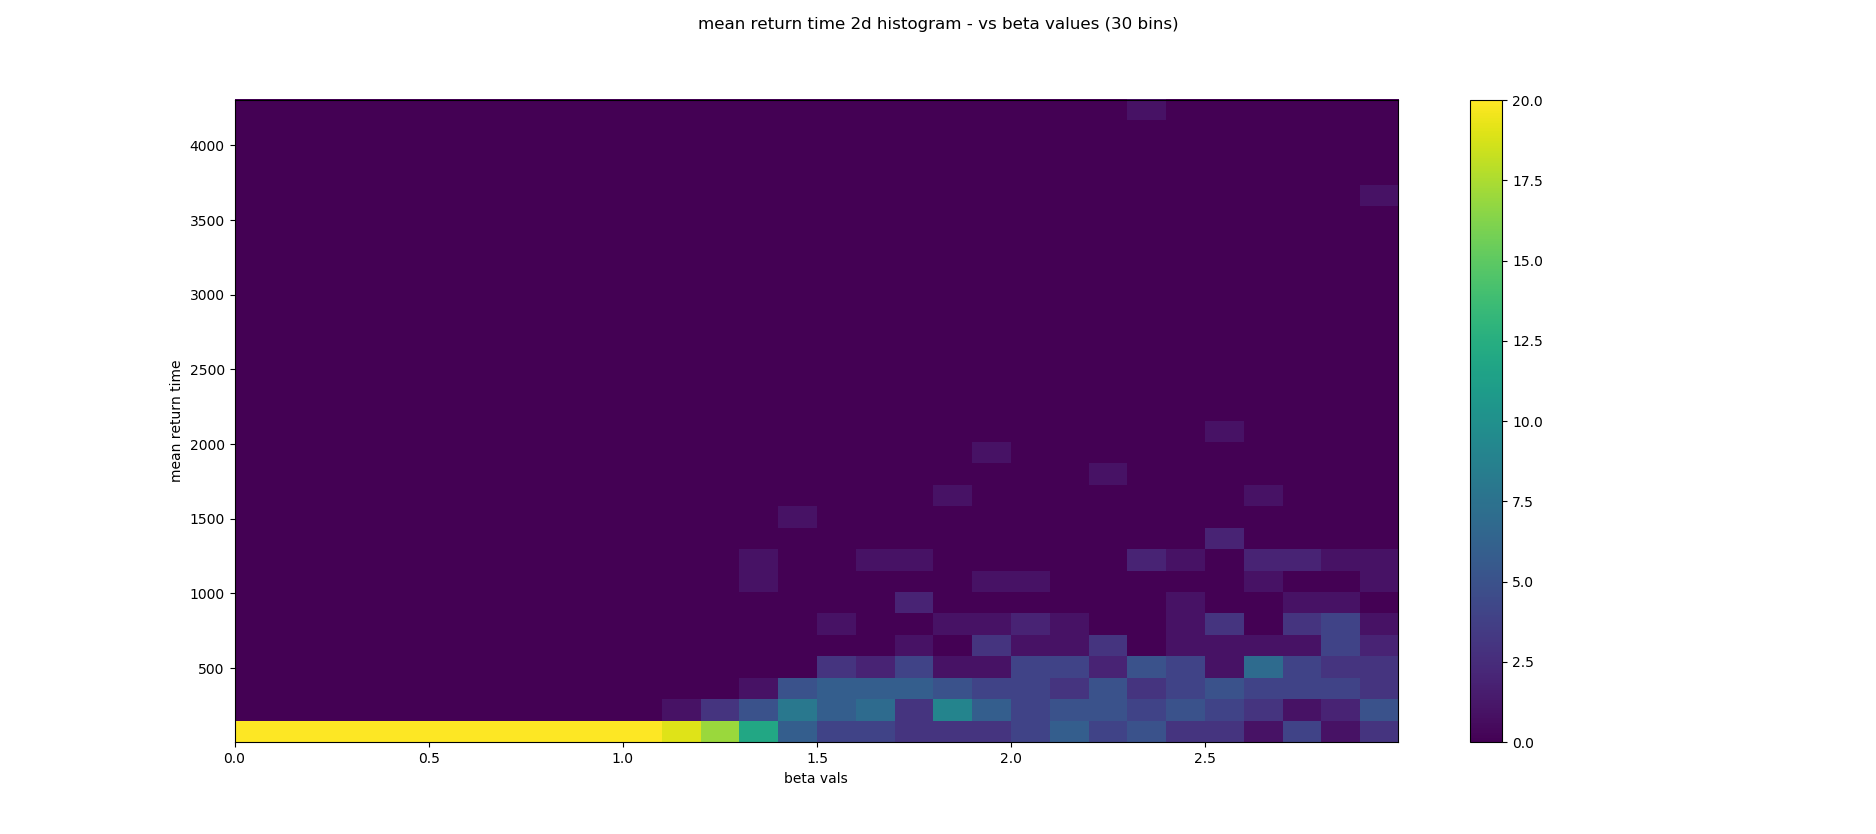
\includegraphics[width=\textwidth]{plots/returntimesplot2.png}
    \end{center}
\end{figure}

However, this is not evidence enough to support the claim, especially in mathematics where the standard
of proof lies beyond statistical inference. As such, I turned my attention toward proving the
conjucture, using a variety of analytical tools. According to Kobayashi's \emph{Probability, Random
Processes, and Statistical Analysis}, we mathematically define a recurrent or transient state the
following way. Begin by defining the \emph{first-passage time} $T_{ij}$ as the number of time steps it
takes for the chain to transition from state $i$ to state $j$. Then, we let $\rho_{ij}^{(n)}$ be the
probability that $T_{ij} = n$; in other words, $\rho_{ij}^{(n)} = P(T_{ij} = n)$. Thus, the follwing sum
\[
    \rho_{ij} = \sum_{n=1}^{\infty} \rho_{ij}^{(n)}  
\]
represents the probability that the chain ever starts at state $i$ and transitions to state $j$. Of
particular importance is the quantity $\rho_{ii}$, the probability that the chain ever returns to state
$i$ after first beginning there. From this, we can classify states.
\begin{definition}
    A state $i$ in the state space $\mathcal{S}$ is \emph{transient} if $\rho_{ii} < 1$ and is
    \emph{recurrent} if $\rho_{ii} = 1$.
\end{definition}
However, computation of $f_{ii}$ for any fixed state $i$ proved difficult with the distribution given
above.  Unfortunately, the position-dependence of $p(x)$ and $q(x)$ make combinatoric approaches highly
challenging, and I had to turn my attention elsewhere.

Observe, first, that $p(x) = q(-x)$ when $x > 0$. As a result, the birth and death chain is symmetric
about the origin. Further, since states change in integer increments, if the chain begins to observe
positive values, it must do so at least until the chain returns to the origin. Due to these two facts,
the given birth and death chain can be considered as if it had state space $\N$ instead of $\Z$. Thus,
it suffices to consider the birth and death chain on $\N$ with probability distribution given by
\[
    p(x) = \begin{cases}
        1 & \text{if } x = 0 \\
        \frac{1}{2+x^{-\beta}} & \text{if } x > 0
    \end{cases},
\]
and $q(x) = 1 - p(x)$. In particular, $p(0) = 1$ since $r(0) = 0$ and $q(0) = 0$ by definition.

Importantly, a new concept must be introducted: that of \emph{communication} between states. The
definition comes from Kobayashi.
\begin{definition}
    Let $i$ and $j$ be states. State $j$ is \emph{reachable} from state $i$ if there exists some $m \in
    \N$ so that the quantity $P_{ij}^{(m)} = \P[X_{n+m} = j \mid X_n =i] > 0$, and is denoted $i \to j$.
    If $i \to j$ and $j \to i$, then the states $i$ and $j$ \emph{communicate}, denoted $i
    \leftrightarrow j$.
\end{definition}
It is a common fact of Markov chains that the relation defined by communication is an equivalence
relation on the state space. Further, it is another common fact that all states in a particular
equivalence class defined by communication must be of the same type. This is to say that if $i$ and $j$
belong to the same equivalence class $\mathcal{C}$, and $i$ is a recurrent state, then $j$ is also a
recurrent state (or vice-versa). Further, we define the concept of \emph{irreducibility}.
\begin{definition}
    Let $\mathcal{C}$ be a set of states. $\mathcal{C}$ is \emph{irreducible} if $i \leftrightarrow j$
    for every $i$ and $j$ in $\mathcal{C}$.
\end{definition}

I claim that the birth and death chain with the given probability distribution is an irreducible chain.
\begin{proposition}
    The birth and death chain with probability distribution given by
    \[
        p(x) = \begin{cases}
            1 & \text{if } x = 0 \\
            \frac{1}{2+x^{-\beta}} & \text{if } x > 0
        \end{cases},
    \]
    $q(x) = 1-x$ and $r(x) = 0$ is irreducible.
\end{proposition}
\begin{proof}
    Note that for every state $i$ with $i > 0$, the quantities $p(i)$ and $q(i)$ are both positive.
    Now, fix arbitrary states $i$ and $j$, and without loss of generality suppose that $j > i$ and that
    $i \neq 0$ and $j \neq 0$. We wish to show that there exists some $m$ so that $P_{ij}^{(m)} =
    \P[X_{n+m} = j \mid X_n = i]$. Let $m = j-i$. Then, 
    \[
        P_{ij}^{(m)} = p(i)\, p(i+1)\, p(i+2)\, \cdots \, p(i+(j-i)).
    \]
    However, since all terms in this product are positive, so must be the product, so that $P_{ij}^{(m)}
    > 0$, so that $i \to j$. Similarly,
    \[
        P_{ji}^{(m)} = q(j)\, q(j-1)\, q(j-2) \, \cdots \, q(j-(j-i)),
    \]
    which is also positive, so that $j \to i$. Thus, $i \leftrightarrow j$ when $i$ and $j$ are
    positive. Now, suppose that $i = 0$. Since it has been determined that $1 \leftrightarrow j$, it
    suffices to show that $0 \leftrightarrow 1$. Trivially, $p(0) = 1$ and $q(1) = 2/3$, so that $0
    \leftrightarrow 1$. Since $\leftrightarrow$ defines an equivalence relation, it follows that $0
    \leftrightarrow j$ for any $j$. Thus, the chain must be irreducible.
\end{proof}

Since the chain is irreducible, every state in the chain must share the same recurrence-classification.
This is to say that all states are either transient, null-recurrent, or positive-recurrent. This allows
the use of the following fact, from Zhong Li.
\begin{proposition}
    An arbitrary birth and death chain on $\N$ with probability distribution defined by $p(x)$ and
    $q(x)$ is transient if and only if
    \[
        \sum_{x = 1}^{\infty} \frac{q(1)\,q(2)\,q(3)\,\cdots\,q(x)}{p(1)\,p(2)\,p(3)\,\cdots\,p(x)} <
        \infty.  
    \]
\end{proposition}
\begin{proof}
    Proof forthcoming.
\end{proof}

Thus, we can prove the following proposition.
\begin{proposition}
    The power-distributed birth and death chain with parameter $\beta$ is recurrent for any $\beta$.
\end{proposition}
\begin{proof}
    It suffices to show that the sum
    \[
        \sum_{x = 1}^{\infty} \frac{q(1)\,q(2)\,q(3)\,\cdots\,q(x)}{p(1)\,p(2)\,p(3)\,\cdots\,p(x)}
    \]
    diverges. Note that for any state $i$, $q(i) = 1-p(i)$. Thus,
    \[
        q(i) = 1 - \frac{1}{2 + i^{-\beta}} = \frac{1 + i^{-\beta}}{2 + i^{-\beta}}.  
    \]
    Thus, the sum simplifies, so that
    \[
        \sum_{x = 1}^{\infty} \frac{q(1)\,q(2)\,q(3)\,\cdots\,q(x)}{p(1)\,p(2)\,p(3)\,\cdots\,p(x)} =
        \sum_{x = 1}^{\infty} (1+1^{-\beta})\,(1+2^{-\beta})\,\cdots\,(1 + x^{-\beta}).
    \]
    The summand is clearly larger than $1$, so that the series must diverge. Thus, the chain is
    recurrent.
\end{proof}

However, we must still show that the chain is positive-recurrent for values of $\beta < 1$ and
null-recurrent for values of $\beta \geq 1$. Doing so will involve the use logarithms and approximations
thereof, as well as a key observation about Riemann sums in relation to corresponding integrals.
Further, we draw upon a second of Zhong Li's results:
\begin{proposition}
    An arbitrary birth and death chain on $\N$ with probability distribution defined by $p(x)$ and
    $q(x)$ is positive-recurrent if and only if
    \[
        \sum_{x=1}^{\infty} \frac{p(0)\, p(1)\, p(2)\, \cdots\, p(x-1)}{q(1)\, q(2)\, q(3)\, \cdots \,
        q(x)} < \infty.  
    \]
\end{proposition}
\begin{proof}
    Proof Forthcoming
\end{proof}
\begin{proposition}
    The power-distributed birth and death chain with parameter $\beta$ is positive-recurrent if $\beta
    < 1$.
\end{proposition}
\begin{proof}
    Let $B$ denote the value
    \[
        \sum_{x=1}^{\infty} \frac{p(0)\, p(1)\, p(2)\, \cdots\, p(x-1)}{q(1)\, q(2)\, q(3)\, \cdots \,
        q(x)}.
    \]
    It suffices to show that $B < \infty$. Note that,
    \[
        q(x) = 1 - p(x) = \frac{1+x^{-\beta}}{2+x^{-\beta}}.
    \]
    Therefore, we can rewrite $B$ as
    \[
        B = \sum_{x=1}^{\infty} \frac{2+x^{-\beta}}{(1+1^{-\beta})\, (1+2^{-\beta})\, \cdots \,
        (1+x^{-\beta})}.  
    \]
    Now, we may leverage a useful property of logarithms: that they can ``convert'' products to sums. In
    particular, it is true that
    \[
        \log\left((1+1^{-\beta})\, (1+2^{-\beta})\, \cdots \, (1+x^{-\beta})\right) = \sum_{i=1}^x
        \log\left(1+i^{-\beta}\right).
    \]
    Further, it is true that for any choice of $\beta$ and for every $i \geq 1$,
    \[
        \frac{1}{4} i^{-\beta} \leq \log\left(1+i^{-\beta}\right).
    \]
    Thus, we have that
    \[
        \log\left((1+1^{-\beta})\, (1+2^{-\beta})\, \cdots \, (1+x^{-\beta})\right) \geq
        \frac{1}{4}\sum_{i=1}^x i^{-\beta}.
    \]
    Let
    \[
        s(x) = \sum_{i=1}^x i^{-\beta}.
    \]
    We now make the key observation that this sum is a Riemann-sum with rectangular width of $1$
    approximating the integral of the function $f(i) = i^{-\beta}$. This is to say that
    \[
        s(x) \approx \int_1^{x+1} i^{-\beta} \, \d i,
    \]
    and that $s(x)$ is the left-endpoint Riemann sum. Notice that $f$ is a strictly decreasing function
    for positive $i$. As a result, we know that the left-endpoint Riemann sum must be greater than or
    equal to the value of the appropriate integral, which is to say that
    \[
        s(x) \geq \int_1^{x+1} i^{-\beta} \, \d i = \frac{1}{1-\beta}\left((x+1)^{1-\beta} - 1\right).
    \]
    Thus, tying this all together---particularly by utilizing the fact that the exponential is an
    increasing function and thus maintains inequalities---shows that
    \[
        \log\left((1+1^{-\beta})\, (1+2^{-\beta})\, \cdots \, (1+x^{-\beta})\right) \geq \exp(s(x)) \geq
        c \,\exp\left(\frac{(x+1)^{1-\beta}}{1-\beta}\right),
    \]
    where
    \[
        c = \exp\left(-\frac{1}{1-\beta}\right).  
    \]
    Therefore, we can now estimate the value $B$ by noting that
    \[
        B \leq \sum_{x=1}^{\infty} \frac{2+x^{-\beta}}{c\,
        \exp\left(\frac{(x+1)^{1-\beta}}{1-\beta}\right)} \leq \sum_{x=1}^{\infty} \frac{3}{c\,
        \exp\left(\frac{(x+1)^{1-\beta}}{1-\beta}\right)}.
    \]
    Finally, since $0 < \beta < 1$, then the function
    \[
        g(x) = \frac{(1+x)^{1-\beta}}{1-\beta}
    \]
    is increasing, so that the denominator in the final sum is an exponential of an increasing function.
    As a result, it can be concluded that
    \[
        \sum_{x=1}^{\infty} \frac{3}{c\, \exp\left(\frac{(x+1)^{1-\beta}}{1-\beta}\right)} < \infty,
    \]
    which shows that $B$ is finitely-valued. Therefore, when $\beta < 1$, the birth and death chain is
    positive-recurrent.
\end{proof}
